\chapter{Experiment and Result}
brief of experiment and result. Chapter 4

\section{Teori}
\section{Tasya Wiendhyra/1164086}
Hari Pertama Minggu Keempat
\subsection{Klasifikasi Teks}
\subsubsection{Pengertian Dan Ilustrasi}
Merupakan salah satu tugas terpenting dalam Pemrosesan Bahasa Alami (Natural Language Processing). Ini adalah proses mengklasifikasikan string teks atau dokumen ke dalam kategori yang berbeda, tergantung pada konten string. Klasifikasi teks memiliki berbagai aplikasi, seperti mendeteksi sentimen pengguna dari tweet, mengklasifikasikan email sebagai spam atau ham, mengklasifikasikan posting blog ke dalam kategori yang berbeda, penandaan otomatis permintaan pelanggan, dan sebagainya. BErikut adalah contoh dari Klasifikasi Teks.\\
Contohnya, misal kita ingin mencari kata dog, table, on, the . kemudian jika kata yang dimaksud sesuai maka akan menampilkan bilangan biner 1 dan jika salah 0. Seperti dibawah ini :
\begin{figure}[ht]
\centering
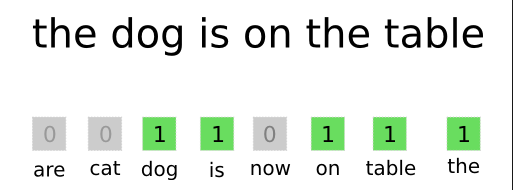
\includegraphics[scale=0.5]{figures/chapter4tasya1.png}
\caption{Klasifikasi Teks Tasya}
\label{Contoh}
\end{figure}
\\
\\
\\
\\
\subsection{Klasifikasi Bunga}
Jelaskan mengapa klasifikasi bunga tidak bisa menggunakan machine learning, sertakan ilustrasi sendiri.\\
Dikarenakan tidak semua bunga memliki ciri - ciri yang sama. Atau dalam kata lain terdapat data noise dalam klasifikasi bunga sehingga tidak bisa menggunakan machine learning.\\
Contohnya Anggrek memiliki warna ungu, dengan jumlah kelopak 5. Kemudian ada bunga warna ungu dengan jumlah kelopak yang sama namun ternyata bukan anggrek dan kategorinya banyak sekali. Bahkan ada bunga yang tidak jelas apakah warnanya sesuai atau tidak, sehingga bisa menyebabkan data noise.
\begin{figure}[ht]
\centering
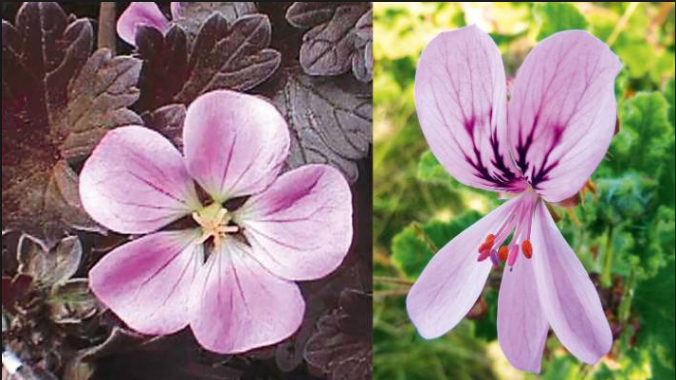
\includegraphics[scale=0.5]{figures/chapter4tasya2.png}
\caption{Klasifikasi Bunga Berwana Ungu Tasya}
\label{Contoh}
\end{figure}

\subsection{Pembelajaran Mesin Pada Teks Kata - Kata di Youtube}
Menggunakan teknik bag-of-words pada klasifikasi berbasis text dan kata untuk mengklasifikasikan komentar yang ada di internet sebagai spam atau bukan. Misalkan pada kolom komentar dapat di cek seberapa sering suatu kata muncul dalam kalimat. Setiap kata dapat dijadikan baris dan kolomnya ini merupakan kategori kata terbut, apakah masuk kedalam spam atau tidak. dan contoh lainnya yaitu pada Caption. dimana akan muncul subtitle secara otomatis dari youtube menggunakan sensor suara yang disesuaikan dengan kata yang telah ditentukan. Contohnya seperti berikut :
\begin{figure}[ht]
\centering
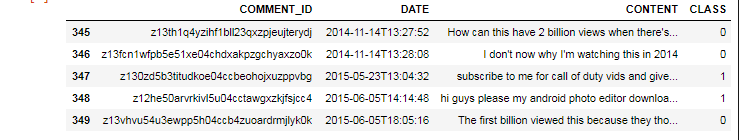
\includegraphics[scale=0.5]{figures/chapter4tasya3.png}
\caption{Klasifikasi Comment Spam Di Youtube Tasya}
\label{Contoh}
\end{figure}

\subsection{Arti Score 44\% Pada Random Forest, 27\% Pada Decission Tree Dan 29\% Dari SVM}
Itu merupakan presentase keakurasian prediksi yang dilakukan pada saat testing menggunakan label pada dataset yang digunakan. Score merupakan mendefinisikan aturan evaluasi model. Maka pada saat dijalankan akan muncuk persentase tersebut yang menunjukan keakurasian atau keberhasilan dari prediksi yang dilakukan. Jika menggunakan Random Forest maka hasilnya 40\% , jika menggunakan Decission Tree hasil prediksinya yaitu 27\% dan pada SVM 29\% .

\subsection{Bag of Words}
\subsubsection{Pengertian Dan Ilustrasi}
Merupakan representasi teks yang menggambarkan kemunculan kata-kata dalam dokumen. ePngelompokan kata kata kedalam perhitunga, berapakali sebuah kata muncul dalam satu kalimat. Disebut "tas" kata-kata, karena informasi tentang susunan atau struktur kata dalam dokumen dibuang. Model ini hanya berkaitan dengan apakah kata-kata yang diketahui muncul dalam dokumen, bukan di mana dalam dokumen.\\
Contohnya disini akan melihat kemunculan kata dari kalimat :
\begin{enumerate}
\item I Love Dogs
\item I hate dogs and knitting
\item Knitting is my hobby and passion. 
\end{enumerate}
\begin{figure}[ht]
\centering
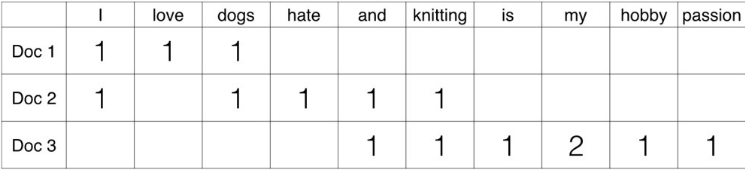
\includegraphics[scale=0.5]{figures/chapter4tasya4.png}
\caption{Bag of Words Tasya}
\label{Contoh}
\end{figure}

\subsection{TF-IDF}
\subsubsection{Pengertian Dan Ilustrasi}
TF-IDF  memberi kita frekuensi kata dalam setiap dokumen dalam korpus atau mengganti data jadi number. Ini adalah rasio berapa kali kata itu muncul dalam dokumen dibandingkan dengan jumlah total kata dalam dokumen itu. Itu meningkat seiring jumlah kemunculan kata itu di dalam dokumen meningkat. Setiap dokumen memiliki tf sendiri. Dalam ilustrasi disini saya akan mengganti contoh Bag of Words menjadi bentuk TF-IDF.
\begin{figure}[ht]
\centering
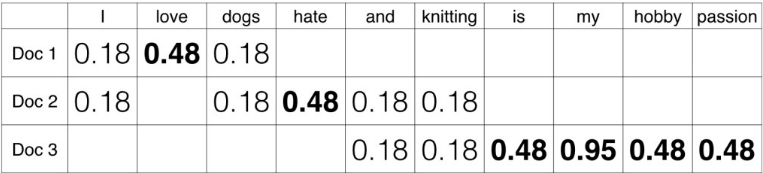
\includegraphics[scale=0.5]{figures/chapter4tasya5.png}
\caption{Contoh TF-IDF Tasya}
\label{Contoh}
\end{figure}

\section{Annisa Fathoroni/1164067}
\subsection{Teori}
Penjelasan Tugas Harian 7 ( No 1-6 )
\begin{enumerate}
\item Pengertian Klasifikasi Teks Dan Ilustrasi Gambar
\begin{itemize}
\item Pengertian

Klasifikasi teks digunakan untuk mengelompokkan teks ke dalam grup yang terorganisir. Teks dianalisis oleh model dan kemudian tag yang sesuai diterapkan berdasarkan konten. Model pembelajaran mesin yang dapat secara otomatis menerapkan tag untuk klasifikasi dikenal sebagai pengklasifikasi.

\item Ilustrasi Gambar

Berdasarkan pengertian diatas, ada beberapa contoh yang bisa diterapkan. Untuk salah satu contoh dari klasifikasi data sendiri dapat diliat pada gambar berikut:

\begin{figure}[!hbtp]
\centering
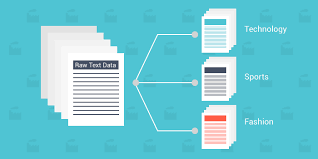
\includegraphics[scale=0.8]{figures/Chapter4AnnisaFathoroni1.png}
\caption{Klasifikasi Text - Annisa Fathoroni}
\label{Klasifikasi Text - Annisa Fathoroni}
\end{figure}

\end{itemize}

\item Mengapa Klasifikasi Bunga Tidak Bisa Menggunakan Machine Learning Dan Ilustrasi Gambar
\begin{itemize}
\item  Penjelasan

Untuk klasifikasi bunga tidak dapat menggunakan machine learning dikarenakan memiliki masalah input yang serupa namun output yang berbeda, biasanya output / error ini disebut dengan istilah 'noise'. Noise sendiri merupakan output yang disimpan/ditangkap ataupun direkam bukan seperti seharusnya ( keluaran yang diiginkan ). Apabila diberikan contoh, maka mari kita misalkan sebuah contoh. Contohnya yaitu kita berasumsi secara implisit bahwa klarifikasi bunga kita sudah tepat seperti kita ahli tanaman. Namun terjadi masih terjadi kesalahan. Selain itu, selalu ada peluang untuk memperkenalkan kesalahan saat merekam data. Maka harus dilakukan penelitian yang lebih rinci sehingga tidak menimbulkan 'noise' itu sendiri.

\item Ilustrasi Gambar

Berdasarkan pengertian diatas, ada beberapa contoh yang bisa diterapkan. Untuk salah satu contoh dari klasifikasi bunga sendiri dapat diliat pada gambar berikut.

\begin{figure}[!hbtp]
\centering
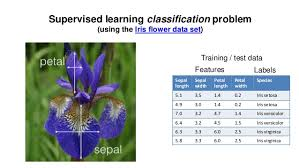
\includegraphics[scale=0.8]{figures/Chapter4AnnisaFathoroni2.jpg}
\caption{Klasifikasi Bunga Machine Learning - Annisa Fathoroni}
\label{Klasifikasi Bunga Machine Learning - Annisa Fathoroni}
\end{figure}

\end{itemize}

\item Teknik Pembelajaran Mesin Pada Teks Pada Kata-Kata Yang Digunakan Di Youtube Dan Ilustrasi Gambar
\begin{itemize}
\item  Penjelasan

Kita ambil sebuah kasus yang semua orang telah ketahui dan juga pahami. Kasus tersebut yaitu perekomendasian video dari pencarian menggunakan "text / kata" di  Youtube. Pada saat menggunakan Youtube terdapat Mchine Learning yang bekerja dan memproses perintah ataupun aktivitas tersebut, dimana akan memfilter secara otomatis video yang disesuaikan dengan "keyword" yang kita masukkan sehingga memberikan keluaran video dengan keyword yang benar. Adapula pada saat kita sedang menonton video di YouTube, pada bagian sebelah kanan ( tampilan Youtube ) terdapat 'Up Next' yang menampilkan beberapa video serupa yang sedang ditonton. Dan ketika mengklik salah satu video dari baris tersebut, maka YouTube akan mengingatnya dan menggunakan kata yang tertera sebagai referensi kembali sehingga akan memberikn kemudahan pada pencarian yang lannya, Dan disitulah mesin belajar sendiri dan menyimpan data secara berkala sehingga berkembang. 

\item Ilustrasi Gambar

Berdasarkan pengertian diatas, ada beberapa contoh yang bisa diterapkan. Untuk salah satu contoh dari Mesin Teks Youtube sendiri dapat diliat pada gambar berikut.

\begin{figure}[!hbtp]
\centering
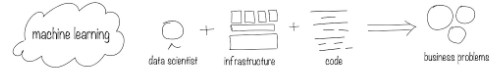
\includegraphics[scale=0.8]{figures/Chapter4AnnisaFathoroni3.jpeg}
\caption{Teknik Pembelajaran Mesin - Annisa Fathoroni}
\label{Teknik Pembelajaran Mesin - Annisa Fathoroni}
\end{figure}

\end{itemize}

\item Vektorisasi Data
\begin{itemize}
\item Penjelasan

Pembagian dan pemecahan data, kemudian dilakukan perhitungan. Vektorisasi juga dapat dimaksudkan dengan setiap data yang mungkin dipetakan ke integer tertentu. jika kita memiliki array yang cukup besar maka setiap kata / data cocok dengan slot unik dalam array (nilai pada indeks adalah nomor satu kali kata itu muncul).

Array angka floating point.

Mewakili data:

\begin{itemize}
\item teks
\item audio
\item gambar
\end{itemize}

Contoh : -[1.0, 0.0, 1.0, 0.5]

\end{itemize}


\item Pengertian Bag Of Words Dan Ilustrasi Gambar
\begin{itemize}
\item  Penjelasan

Bag-of-words ialah sebuah gambaran sederhana digunakan dalam pengolahan bahasa alami dan pencarian informasi. Dikenal sebagai model ruang vektor. Pada model ini, tiap kalimat dalam dokumen digambarkan sebagai token, mengabaikan tata bahasa dan bahkan urutan kata namun menghitung frekuensi kejadian atau kemunculan kata dari dokumen.

\item Ilustrasi Gambar

Berdasarkan pengertian diatas, ada beberapa contoh yang bisa diterapkan. Untuk salah satu contoh dari Bag Of Words sendiri dapat diliat pada gambar berikut.

\begin{figure}[!hbtp]
\centering
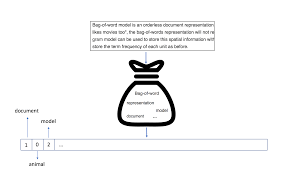
\includegraphics[scale=0.8]{figures/Chapter4AnnisaFathoroni4.png}
\caption{Bag of Words - Annisa Fathoroni}
\label{Bag of Words - Annisa Fathoroni}
\end{figure}

\end{itemize}

\item Pengertian TF-IDF Dan Ilustrasi Gambar
\begin{itemize}
\item  Penjelasan

TF-IDF merupakan metode untuk menghitung bobot setiap kata yang paling umum digunakan pada information retrieval. Metode ini juga terkenal efisien, mudah dan memiliki hasil yang akurat. Metode ini akan menghitung nilai Term Frequency (TF) dan Inverse Document Frequency (IDF) pada setiap token (kata) di setiap dokumen dalam korpus

\item Ilustrasi Gambar

Berdasarkan pengertian diatas, ada beberapa contoh yang bisa diterapkan. Untuk salah satu contoh dari TF-IDF sendiri dapat diliat pada gambar berikut.

\begin{figure}[!hbtp]
\centering
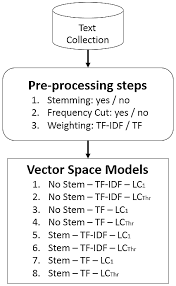
\includegraphics[scale=0.8]{figures/Chapter4AnnisaFathoroni5.png}
\caption{TF IDF - Annisa Fathoroni}
\label{TF IDF - Annisa Fathoroni}
\end{figure}

\end{itemize}

\end{enumerate}


\section{Annisa Cahyani-1164066}
\subsection{Teori}
Penjelasan Tugas Harian ke- 7 ( No 1-6 )
\begin{enumerate}
\item Pengertian Klasifikasi Teks Dan Ilustrasi Gambar
\begin{itemize}
\item Pengertian Klasifikasi Teks
\par Klasifikasi teks atau kategorisasi teks merupakan suatu proses yang secara otomatis menempatkan dokumen teks tersebut ke dalam suatu kategori yang berdasarkan dengan isi dari teks tersebut proses pemberian tag atau kategori pada teks harus sesuai dengan isinya. 
\par
\end{itemize}
\par
\par
\item Mengapa Klasifikasi Bunga Tidak Bisa Menggunakan Machine Learning Dan Ilustrasi Gambar
\begin{itemize}
\item  Mengapa Klasifikasi Bunga Tidak Bisa Menggunakan Machine Learning
\par Mengapa untuk pengklasifikasi pada bunga tidak dapat menggunakan machine learning karena memiliki masalah input yang serupa tetapi menggunakan output yang berbeda, biasanya output atau error ini biasa  disebut dengan istilah 'noise'. Noise adalah output yang disimpan atau yang ditangkap ataupun yang direkam bukan seperti seharusnya ( keluaran yang diiginkan ). 
\par
\end{itemize}
\par
\par
\item Teknik Pembelajaran Mesin Pada Teks Pada Kata-Kata Yang Digunakan Di Youtube Dan Ilustrasi Gambar
\begin{itemize}
\item  Teknik Pembelajaran Mesin Pada Teks Pada Kata-Kata Yang Digunakan Youtube
\par Yaitu ambil sebuah kasus yang  dimana semua orang telah mengetahui dan juga memahaminya. Kasus yang dimaksud  yaitu perekomendasian video dari sebuah  pencarian dengan menggunakan "text atau kata" pada  Youtube. Yang dimana pada saat kita menggunakan Youtube terdapat Mchine Learning yang akan bekerja dan mulai memproses perintah ataupun aktivitas tersebut, yang  dimana akan memfilter secara otomatis video-video yang telah disesuaikan dengan "keyword" yang telah kita masukkan sehingga dapat memberikan keluaran video dengan keyword yang sesuai.  
\par
\end{itemize}
\par
\par
\item Vektorisasi Data
\begin{itemize}
\item Maksud Dari Vektorisasi Data
\par Pada pembagian atau pemecahan data, yang dilakukan adalah perhitungan. Vektorisasi juga dapat diartikan dengan setiap data yang telah mungkin dipetakan ke integer yang  tertentu. Apabila memiliki array yang cukup besar maka setiap kata  atau data yang ada dan cocok dengan slot unik dalam array maka nilai yang ada pada indeks tersebut adalah nomor satu kali kata itu muncul.
\par
\end{itemize}
\par
\par
\item Pengertian Bag Of Words Dan Ilustrasi Gambar
\begin{itemize}
\item  Pengertian Bag Of Words
\par Bag of words adalah merupakan representasi penyederhanaan yang digunakan dalam  suatu pemrosesan bahasa yang alami dan pengambilan suatu informasi. Dalamnya yaitu sebuah teks yang seperti kalimat atau dokumen yang  mewakili sebagai tas (multiset) dari kata-katanya, mengabaikan tata bahasa dan bahkan urutan kata tetapi tetap menjaga multiplisitas.
\par
\end{itemize}
\par
\par
\item Pengertian TF-IDF Dan Ilustrasi Gambar
\begin{itemize}
\item  Pengertian TF-IDF
\par TF-IDF merupakan salah satu dari metode yang biasa digunakan untuk melakukan pembobotan kata sebelum melakukan suatu  proses selanjutnya. Biasanya pembobotan kata ini akan diperlukan jika kita ingin melakukan sebuah  pemrosesan Bahasa alami atau pembuatan system temu kembali informasi. 
\par
\end{itemize}
\par
\par
\end{enumerate}